\documentclass[10pt,aspectratio=169]{beamer}

% All the boilerplate is in ccaslides.sty
% Note that this also pulls in a custom vogtwidebar.sty
\usepackage{ccaslides}

\author{Ji\v{r}\'i Lebl}

\institute[OSU]{%
Departemento pri Matematiko de Oklahoma {\^S}tata Universitato}

\title{Cultivating Complex Analysis:\\%
Riemann mapping theorem (6.3.1)}

\date{}

\begin{document}

\begin{frame}
\titlepage
\end{frame}

\begin{frame}
Riemann mapping theorem: The only simply connected domains in
$\C$ (up to biholomorphisms) are $\C$ and $\D$.

\pause
\medskip

More precisely:

\begin{theorem}[Riemann mapping theorem]
Let $U \subset \C$ be a simply connected domain such that $U \not= \C$.
Let $p \in U$ be given.  Then there exists a unique biholomorphic (conformal)
map $f \colon U \to \D$ such that $f(p) = 0$ and
$f'(p) > 0$.
\end{theorem}

\medskip
\pause

$U={}$ the upper half disk

$p=(\sqrt{2}-1)i$

\vspace*{-\baselineskip}

\hspace*{1in}
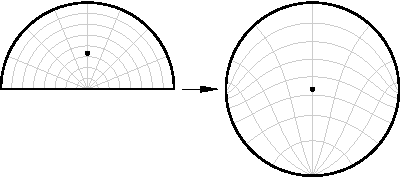
\includegraphics{../figures/riemannmap}

\pause

Proof is to ``maximize'' $\sabs{f'(p)}$ among all maps into the disc and $f(p)=0$.


\end{frame}

\begin{frame}
\begin{theorem}[Riemann mapping theorem]
Let $U \subset \C$ be a simply connected domain such that $U \not= \C$.
Let $p \in U$ be given.  Then there exists a unique biholomorphic
map $f \colon U \to \D$ such that $f(p) = 0$ and
$f'(p) > 0$.
\end{theorem}

\pause


\textbf{Proof:}
Let $\sF$ be the set of injective holomorphic $f \colon U \to \D$ such that $f(p) = 0$. 

\pause
\medskip

First we need to prove that $\sF$ is nonempty:

\medskip
\pause

Let $q \in \C \setminus U$.
\quad
\pause
$\exists$ $g \colon U \to \C$ such that ${\bigl(g(z)\bigr)}^2 = z-q$
\quad ($U$ simply connected).

\medskip

\pause
$g(z)=g(\zeta)$
\pause
\wthus
${\bigl(g(z)\bigr)}^2={\bigl(g(\zeta)\bigr)}^2$
\pause
\wthus
$z=\zeta$
\pause
\wthus
$g$ is injective.

\medskip

\pause
$g(z)=-g(\zeta)$
\pause
\wthus
${\bigl(g(z)\bigr)}^2={\bigl(g(\zeta)\bigr)}^2$
\pause
\wthus
$z=\zeta$
\pause
\wthus
contradiction
($g$ is never zero).

\pause
\thus\quad
$g(U) \cap \bigl( - g(U) \bigr) = \emptyset$
\quad
where
$-g(U) = \{ z \in \C : -z \in g(U) \}$.

\medskip
\pause

$g(U)$ is open
\pause
\wthus
$-g(U)$ is open
\pause
\wthus $\exists$ $\Delta_r(\xi) \subset  \C \setminus g(U)$

\medskip

\pause
\thus \quad
$z \mapsto \dfrac{r}{g(z)-\xi}$
\quad
takes $U$ to $\D$.

\medskip

\pause
Compose with an automorphism of $\D$ to make $p$ go to $0$
\pause
\wthus
$\sF$ is nonempty.
\end{frame}

\begin{frame}
Suppose $f \colon U \to \D$ is in $\sF$ but not onto.
\pause
~
Suppose $q \in \D \setminus f(U)$.

\pause
Let $\varphi_q(z) = \dfrac{z-q}{1-\bar{q}z}$.
\quad
Note $\varphi_q \in \Aut(\D)$, \quad $\varphi_q(q)=0$, \quad
and $\varphi_q \circ f$ nonzero.

\pause
$\exists$ $g \colon U \to \C$ s.t.
${\bigl(g(z)\bigr)}^2 = \varphi_q\bigl(f(z)\bigr)$.
\pause
\quad
$g(U) \subset \D$.
\pause
\quad
$g(z)=g(\zeta)$ \wthus $\varphi_q\bigl(f(z)\bigr)=\varphi_q\bigl(f(\zeta)\bigr)$.

\pause
$\varphi_q \circ f$ injective \wthus $g$ injective.
\quad

\pause
\medskip

Define
$h = \varphi_{g(p)} \circ g$.
\quad \pause
$h(p) =0$ \wthus $h \in \sF$.
\pause
\quad
Also
~$g = \varphi_{-g(p)} \circ h$.

\pause
\medskip

Differentiate
$\varphi_q \circ f = g^2$ at $p$ (recall $\varphi_a'(0) = 1-\sabs{a}^2$):
\pause
\[
\bigl(1-\sabs{q}^2\bigr) f'(p)
= \varphi_q'\bigl(f(p)\bigr) f'(p)
\pause
= 2 g(p) g'(p)
\pause
= 2 g(p) \varphi_{-g(p)}'\bigl(h(p)\bigr) h'(p)
\pause
= 2 g(p) \bigl(1-\sabs{g(p)}^2\bigr) h'(p) .
\]
\pause
$\displaystyle
\sabs{f'(p)} =
\frac{2 \sabs{g(p)} \bigl(1-\sabs{g(p)}^2\bigr)}{1-\sabs{q}^2} \sabs{h'(p)}
\pause
=
\frac{2 \sqrt{\sabs{q}}}{1+\sabs{q}} \sabs{h'(p)}
$
\qquad as
${\bigl(g(p)\bigr)}^2 = -q$.

\pause
\medskip

$\sabs{q} < 1$
\wthus
$\displaystyle \frac{2 \sqrt{\sabs{q}}}{1+\sabs{q}} < 1$
\pause
\wthus
$\displaystyle \sabs{f'(p)} < \sabs{h'(p)}$.
\end{frame}

\begin{frame}
Construct a sequence $\{ f_n \}$ in  $\sF$ such that 
\[
\lim_{n \to \infty} \sabs{f_n'(p)} = \sup_{f \in \sF} \sabs{f'(p)}
\]
\pause
Montel says ($\sF$ is uniformly bounded),
there exists a convergent subsequence,

\pause
WLOG $\{ f_n \}$ converges to $f$.

\medskip
\pause

By the corollary to Hurwitz, $f$ is injective or constant.

\medskip
\pause
By taking limits: $\sabs{f'(p)} > 0$ ($f$ not constant),
\pause
\quad
$f(p) = 0$,
\pause
\quad
$\sabs{f(z)} \leq 1$ for all $z \in U$.

\pause
Open mapping theorem \wthus
$\sabs{f(z)} < 1$ for all $z \in U$.

\medskip
\pause
$f$ must be onto, otherwise there would be an $h \in \sF$ with
$\sabs{f'(p)} < \sabs{h'(p)}$.

\medskip
\pause
Uniqueness left as an exercise. \qed
\end{frame}

\begin{frame}
\textbf{Remark:}
An explicit map is useful, e.g., in differential equations.

\pause
The theorem doesn't answer how a map is constructed.

\pause
There is lots of literature on constructing the map.

\pause
E.g., if $U$ is a polygon, there is an explicit formula:
the Schwarz--Christoffel mapping.

\medskip
\pause

\textbf{Remark:}
The theorem doesn't answer how regular the map is up to the boundary.

\pause
The nicer the boundary, the nicer the map will be.

\end{frame}

\begin{frame}
\textbf{Exercise:}
Suppose $U \subset \C$ is a simply connected domain.
Show that for every two points $z,w \in U$, there exists an automorphism
$\psi \in \Aut(U)$ such that $\psi(z) = w$.

\pause
\medskip

\textbf{Exercise:}

a)
Suppose $U \subset \C$ is a simply connected domain, $U \not= \C$,
$p,q \in U$ are distinct points, and
$f \colon U \to U$ is holomorphic such that $f(p) = p$ and $f(q)=q$.
Prove that $f$ is the identity.

\pause
b)
Find a counterexample if $U=\C$.

\pause
\medskip

\textbf{Exercise:}
Show that $\D \setminus \{ 0 \}$
and the annulus $\ann(0;1,2)$ are not biholomorphic.

\pause
\medskip

\textbf{Exercise:}
Suppose $f \colon \C \to \C$ is entire holomorphic and
injective, prove that $f$ is onto.


\end{frame}

\end{document}
